\documentclass{article}
\usepackage{fancyhdr}
\usepackage{graphicx}
\usepackage{amsmath}
\usepackage{xcolor}
\usepackage{caption}
\usepackage{amssymb}

\usepackage[margin=1in]{geometry}
\usepackage{cancel} 

\pagestyle{fancy}
\graphicspath{ {./img/} }

\begin{document}
	\begin{titlepage}
		\begin{center}
			\vspace{1cm}
			{\LARGE\textbf{741 Operational Amplifier}}
			
			\vspace{1.5cm}
			\textbf{\large Ghassan Arnouk}\\
			
			\vspace{1cm}
			\large ELEC 3509B\\
			\large Summer 2020\\
			\large Lab 3 Report\\
			
			
			\vspace{2cm}
			\textbf{Instructor:} Qi-Jun Zhang\\
			
			
			\vspace{1cm}
			\textbf{Lab Period:} B1\\
			
			\vspace{0.1cm}
			\textbf{Day 1 Preformed:} 2020/07/29
			
			\vspace{0.1cm}
			\textbf{Day 2 Preformed:} 2020/07/30
		
			\vspace{1cm}
			\textbf{Date Submitted:} 2020/08/06\\			
		\end{center}
	\end{titlepage}
	
	\lhead{Ghassan Arnouk (B1)}
	\rhead{741 Op-Amp}
	\pagebreak
	
	\tableofcontents
	\pagebreak
	
	\listoftables
	\pagebreak
	
	\listoffigures
	\pagebreak
	
	\section{Introduction}
	The first amplifying device looked at when studying electronics is the operational amplifier (op-amp). The main purpose of the op-amp is to amplify weak signals when amplified signals are needed. One of the most common op-amps in currently in the market is the 741 op-amp. Along with its ability to amplify signals well, the 741 op-amp is low in cost, thus making it at one point in time, one of the most commonly used devices in electronics.\\
	This lab looks at the 741 op-amp in further detail. The op-amp is analyzed to find its parameters in each transistor within the op-amp and is then simulated on the simulating software PSPICE to compare the measured parameters with the calculated ones. A schematic of the 741 op-amp used in this lab is shown in Figure \ref{f:1} below.
	
	\pagebreak
	\section{Prelab}
	Fig. \ref{f:1} below shows the 741 Operational Amplifier circuit that will analyzed for this prelab.
	\begin{figure}[!ht]
		\centering
		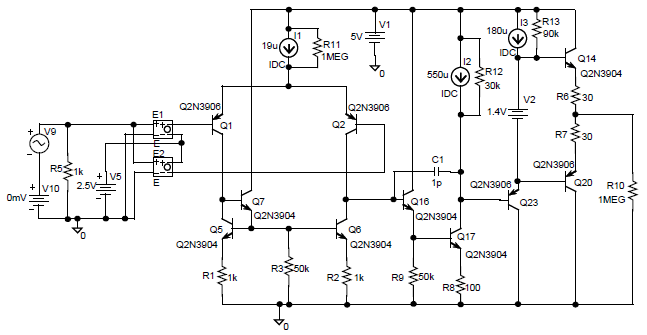
\includegraphics[width=0.7\textheight]{741_op-amp.png}
		\captionof{figure}{741 Operational Amplifier}
		\label{f:1}
	\end{figure}

	\noindent Table \ref{t:1} below lists some assumptions for NPN and PNP parameters that is an asset in completing the prelab calculations.
	\begin{table}[!ht]
		\centering
		\captionof{table}{Assumptions of parameters}
		\begin{tabular}{|c|c|c|}
			\hline
			\textbf{Parameter} & \textbf{NPN} & \textbf{PNP}\\
			\hline\hline
			Early Voltage $V_A$ & 80 V & 20 V\\
			\hline
			Beta (assume constant but note that it normally depends on current) & 100 & 100\\
			\hline
			$I_s$ (recall that $I_c = I_s e^{\frac{V_{BE}}{V_T}}$) & 6.73 fA & 1.41 fA\\
			\hline
			$V_{BE}$ & 0.6 V & 0.6 V\\
			\hline
			$V_{CC}$ & 5 V & 5 V\\
			\hline			
		\end{tabular}
		\label{t:1}
	\end{table}

	\pagebreak
	\subsection{DC Analysis}
	\begin{align*}
		\mathbf{Q_{14} \hspace{2mm} and \hspace{2mm} Q_{20}} \hspace{1mm} \textbf{Transistors}
	\end{align*}
	Applying KVL:
	\begin{align*}
		-1.4 \hspace{1mm} V &= V_{BE_{14}} + R_{6}(I_{R_{10}} + I_{R_{10}}) + R_7 (I_{E_{20}}) + V_{BE_{20}}
	\end{align*}
	By substitution, we get the following:
	\begin{align*}
		1.4 = ln(\frac{I_C}{I_{S_{20}}}) V_T + R_6(I_{E_{20}} + I_{R_{10}}) + R_7 (I_{E_{20}}) + ln(\frac{I_C}{I_{S_{14}}}) V_T
	\end{align*}
	Solving the above equation and ignoring $I_{R_{10}}$, we get the following:
	\begin{align*}
		1.4 \hspace{1mm} V = ln \left[\frac{\left(\frac{100}{101}\right) I_{E_{20}}}{I_{S_{20}}} \right] (25 \hspace{1mm} mV) + (30 \hspace{1mm} \Omega)(I_{E_{20}}) + ln \left[\frac{\left(\frac{100}{101}\right) I_{E_{20}}}{I_{S_{14}}} \right] (25 \hspace{1mm} mV)
	\end{align*}
	\begin{align*}
		\therefore I_{E_{20}} = I_{E_{14}} \approx 1.14 \hspace{1mm} mA
	\end{align*}
	Finding the collector current:
	\begin{align*}
		I_{C_{20}} = I_{C_{14}} &= \frac{\beta}{\beta + 1} (I_{E})\\ 
		&= \frac{100}{100 + 1}(1.14 \hspace{1mm} mA)\\ 
		&\approx 1.13 \hspace{1mm} mA
	\end{align*}
	Finding the transconductance:
	\begin{align*}
		g_{m_{20}} = g_{m_{14}} &= \frac{I_C}{V_T}\\ 
		&= \frac{1.13 \hspace{1mm} mA}{25 \hspace{1mm} mV}\\
		&= 45.2 \hspace{1mm} mA/V
	\end{align*}
	Finding $r_o$:
	\begin{align*}
		r_{o_{20}} &= \frac{V_A}{I_{C_{20}}}\\
		&= \frac{20 \hspace{1mm} V}{1.13 \hspace{1mm} mA}\\
		&= 17.7 \hspace{1mm} k\Omega\\\\
		r_{o_{14}} &= \frac{V_A}{I_{C_{14}}}\\ 
		&= \frac{80 \hspace{1mm} V}{1.13 \hspace{1mm} mA}\\
		&= 70.8 \hspace{1mm} k\Omega
	\end{align*}	
	\pagebreak
	\begin{align*}
		\mathbf{Q_{23}} \hspace{1mm} \textbf{Transistor}
	\end{align*}
	\begin{align*}
		I_{E_{23}} &= \frac{I_{C_{20}}}{\beta} + \left[180 \hspace{1mm} \mu A + \left(\frac{5 \hspace{1mm} V - 3.22 \hspace{1mm} V}{R_{13}} - \frac{I_{C_{14}}}{\beta}\right) \right]\\
		I_{E_{23}} &= \frac{1.13 \hspace{1mm} mA}{100} + \left[180 \hspace{1mm} \mu A + \left(\frac{5 \hspace{1mm} V - 3.22 \hspace{1mm} V}{R_{13}} - \frac{1.13 \hspace{1mm} mA}{100}\right) \right]
	\end{align*}
	\begin{align*}
		\therefore I_{E_{23}} = 200 \hspace{1mm} \mu A
	\end{align*}
	Finding the collector current:
	\begin{align*}
		I_{C_{23}} &= \frac{\beta}{\beta + 1} (I_{E_{23}})\\ 
		&= \frac{100}{100 + 1}(200 \hspace{1mm} \mu A)\\
		&\approx 198 \hspace{1mm} \mu A
	\end{align*}
	Finding the transconductance:
	\begin{align*}
		g_{m_{23}} &= \frac{I_{C_{23}}}{V_T}\\
		&= \frac{198 \hspace{1mm} \mu A}{25 \hspace{1mm} mV}\\
		&= 7.92 \hspace{1mm} mA/V
	\end{align*}
	Finding $r_o$:
	\begin{align*}
		r_{o_{23}} &= \frac{V_A}{I_{C_{23}}}\\
		&= \frac{20 \hspace{1mm} V}{198 \hspace{1mm} \mu A}\\
		&= 101 \hspace{1mm} k\Omega
	\end{align*}
	\begin{align*}
		\mathbf{Q_{17}} \hspace{1mm} \textbf{Transistor}
	\end{align*}
	Finding the collector current:
	\begin{align*}
		I_{C_{17}} &= \frac{I_{C_{23}}}{\beta} + 550 \hspace{1mm}\mu A + \frac{5 \hspace{1mm} V - 1.22 \hspace{1mm} V}{30 \hspace{1mm} k\Omega}\\ 
		&= \frac{198 \hspace{1mm} \mu A}{100} + 550 \hspace{1mm}\mu A + \frac{5 \hspace{1mm} V - 1.22 \hspace{1mm} V}{30 \hspace{1mm} k\Omega}\\ 
		&= 678 \hspace{1mm} \mu A
	\end{align*}
	Finding the transconductance:
	\begin{align*}
		g_{m_{17}} &= \frac{I_{C_{17}}}{V_T}\\
		&= \frac{678 \hspace{1mm} \mu A}{25 \hspace{1mm} mV}\\
		&= 27.1 \hspace{1mm} mA/V
	\end{align*}
	Finding $r_o$:
	\begin{align*}
		r_{o_{17}} &= \frac{V_A}{I_{C_{17}}}\\
		&= \frac{80 \hspace{1mm} V}{678 \hspace{1mm} \mu A}\\
		&= 118 \hspace{1mm} k\Omega
	\end{align*}
	\pagebreak
	\begin{align*}
		\mathbf{Q_{16}} \hspace{1mm} \textbf{Transistor}
	\end{align*}
	Finding the emitter current:
	\begin{align*}
		I_{C_{16}} &= \frac{I_{C_{17}}}{\beta} + \frac{669 \hspace{1mm} mV}{R_9}\\ 
		&= \frac{678 \hspace{1mm} \mu A}{100} + \frac{669 \hspace{1mm} mV}{50 \hspace{1mm} k\Omega}\\ 
		&= 20.2 \hspace{1mm} \mu A
	\end{align*}
	Finding the collector current:
	\begin{align*}
		I_{C_{16}} &= \frac{\beta}{\beta + 1} (I_{E_{16}})\\
		&= \frac{100}{100 + 1} (20.2 \hspace{1mm} \mu A)\\
		&\approx 19.96 \hspace{1mm} \mu A
	\end{align*}
	Finding the transconductance:
	\begin{align*}
		g_{m_{16}} &= \frac{I_{C_{16}}}{V_T}\\
		&= \frac{19.96 \hspace{1mm} \mu A}{25 \hspace{1mm} mV}\\
		&= 798 \hspace{1mm} \mu A/V
	\end{align*}
	Finding $r_o$:
	\begin{align*}
		r_{o_{16}} &= \frac{V_A}{I_{C_{16}}}\\
		&= \frac{80 \hspace{1mm} V}{19.96 \hspace{1mm} \mu A}\\
		&= 4 \hspace{1mm} M\Omega
	\end{align*}
	\begin{align*}
		\mathbf{Q_{1}} \hspace{1mm} \textbf{Transistor}
	\end{align*}
	\begin{align*}
		V_{in} = 2.5 \hspace{1mm} V \rightarrow V_{B_{1}} = 2.5 \hspace{1mm} V\\
		V_{E_{1}} = V_{E_{2}} = 2.5 \hspace{1mm} V + 0.6 \hspace{1mm} V = 3.1 \hspace{1mm} V\\
		\therefore I_{E_1} = I_{E_2} = 10.45 \hspace{1mm} \mu A
	\end{align*}
	Finding the collector current:
	\begin{align*}
		I_{C_{1}} &= \frac{\beta}{\beta + 1} (I_{E_1})\\
		&= \frac{100}{100 + 1} (10.45 \hspace{1mm} \mu A)\\
		&= 10.35 \hspace{1mm} \mu A
	\end{align*}
	Finding the transconductance:
	\begin{align*}
		g_{m_{1}} &= \frac{I_{C_{1}}}{V_T}\\
		&= \frac{10.35 \hspace{1mm} \mu A}{25 \hspace{1mm} mV}\\
		&= 414 \hspace{1mm} \mu A/V
	\end{align*}
	Finding $r_o$:
	\begin{align*}
		r_{o_{1}} &= \frac{V_A}{I_{C_{1}}}\\
		&= \frac{80 \hspace{1mm} V}{10.35 \hspace{1mm} \mu A}\\
		&= 1.93 \hspace{1mm} M\Omega
	\end{align*}
	\begin{align*}
		\mathbf{Q_{2}} \hspace{1mm} \textbf{Transistor}
	\end{align*}
	Finding the collector current:
	\begin{align*}
		I_{C_2} = I_{C_1} = 10.35 \hspace{1mm} \mu A
	\end{align*}
	Finding the transconductance:
	\begin{align*}
		g_{m_2} = g_{m_1} = 414 \hspace{1mm} \mu A/V
	\end{align*}
	Finding $r_o$:
	\begin{align*}
		r_{o_2} = r_{o_1} = 1.93 \hspace{1mm} M\Omega 
	\end{align*}
	\begin{align*}
		\mathbf{Q_6} \hspace{1mm} \textbf{Transistor}
	\end{align*}
	Finding the collector current:
	\begin{align*}
		I_{C_{6}} &= I_{C_2} - \frac{I_{C_{16}}}{\beta}\\
		&= 10.35 \hspace{1mm} \mu A - \frac{19.96 \hspace{1mm} \mu A}{100}\\
		&\approx 10.15 \hspace{1mm} \mu A
	\end{align*}
	Finding the transconductance:
	\begin{align*}
		g_{m_{6}} &= \frac{I_{C_6}}{V_T}\\
		&= \frac{10.15 \hspace{1mm} \mu A}{25 \hspace{1mm} mV}\\
		&= 406 \hspace{1mm} \mu A/V
	\end{align*}
	Finding the $r_o$:
	\begin{align*}
		r_{o_6} &= \frac{V_A}{I_{C_{16}}}\\
		&= \frac{80 \hspace{1mm} V}{10.15 \hspace{1mm} \mu A}\\
		&= 7.9 \hspace{1mm} M\Omega
	\end{align*}
	\pagebreak
	\begin{align*}
		\mathbf{Q_{5}} \hspace{1mm} \textbf{Transistor}
	\end{align*}
	Finding the emitter current:
	\begin{align*}
		I_{E_5} &= \frac{10.25 \hspace{1mm} mV}{R_1}\\
		&= \frac{10.25 \hspace{1mm} mV}{1 \hspace{1mm} k\Omega}\\
		&= 10.25 \hspace{1mm} \mu A
	\end{align*}
	Finding the collector current:
	\begin{align*}
		I_{C_5} &= \frac{\beta}{\beta + 1} (I_{E_5})\\
		&= \frac{100}{100 + 1} (10.25 \hspace{1mm} \mu A)\\
		&\approx 10.15 \hspace{1mm} \mu A
	\end{align*}
	Finding the transconductance:
	\begin{align*}
		g_{m_5} &= \frac{I_{C_5}}{V_T}\\
		&= \frac{80 \hspace{1mm} V}{25 \hspace{1mm} mV}\\
		&= 406 \hspace{1mm} \mu A/V
	\end{align*}
	Finding $r_o$:
	\begin{align*}
		r_{o_6} &= \frac{V_A}{I_{C_{5}}}\\
		&= \frac{80 \hspace{1mm} V}{10.15 \hspace{1mm} \mu A}\\
		&= 7.9 \hspace{1mm} M\Omega
	\end{align*}
	\begin{align*}
		\mathbf{Q_{7}} \hspace{1mm} \textbf{Transistor}
	\end{align*}
	Finding the emitter current"
	\begin{align*}
		I_{E_7} &= \frac{I_{C_5}}{\beta} + \frac{0.61 \hspace{1mm} V}{R_3} + \frac{I_{C_6}}{\beta}\\
		&= \frac{10.15 \hspace{1mm} \mu A}{100} + \frac{0.61 \hspace{1mm} V}{50 \hspace{1mm} k\Omega} + \frac{10.15 \hspace{1mm} \mu A}{100}\\
		&= 12.4 \hspace{1mm} \mu A
	\end{align*}
	Finding the collector current:
	\begin{align*}
		I_{C_7} &= \frac{\beta}{\beta + 1} (I_{E_7})\\
		&= \frac{100}{100 + 1} (12.4 \hspace{1mm} \mu A)\\
		&\approx 12.28 \hspace{1mm} \mu A		
	\end{align*}
	Finding the transconductance:
	\begin{align*}
		g_{m_7} &= \frac{I_{C_7}}{V_T}\\
		&= \frac{12.28 \hspace{1mm} \mu A}{25 \hspace{1mm} mV}\\
		&= 491.2 \hspace{1mm} \mu A/V
	\end{align*}
	Finding $r_o$:
	\begin{align*}
		r_{o_7} &= \frac{V_A}{I_{C_7}}\\
		&= \frac{80 \hspace{1mm} V}{12.28 \hspace{1mm} \mu A/V}\\
		&= 6.5 \hspace{1mm} M\Omega
	\end{align*}
	\begin{table}[!ht]
		\centering
		\captionof{table}{DC Analysis Summary}
		\begin{tabular}{|c|c|c|c|}
			\hline
			Transistor & $I_C$ & $g_m$ & $r_o$\\
			\hline\hline
			$Q_1$ & 10.35 $\mu$A & 414 $\mu$A/V & 1.93 M$\Omega$\\
			\hline
			$Q_2$ & 10.35 $\mu$A & 414 $\mu$A/V & 1.93 M$\Omega$\\
			\hline			
			$Q_5$ & 10.15 $\mu$A & 406 $\mu$A/V & 7.90 M$\Omega$\\
			\hline				
			$Q_6$ & 10.15 $\mu$A & 406 $\mu$A/V & 7.90 M$\Omega$\\
			\hline
			$Q_7$ & 12.28 mA & 491.2 $\mu$A/V & 6.50 M$\Omega$\\
			\hline	
			$Q_{14}$ & 1.13 mA & 45.2 mA/V & 70.8 k$\Omega$\\
			\hline
			$Q_{16}$ & 19.96 $\mu$A & 798 $\mu$A/V & 4 M$\Omega$\\
			\hline			
			$Q_{17}$ & 678 $\mu$A & 27.1 mA/V & 118 k$\Omega$\\
			\hline
			$Q_{20}$ & 1.13 mA & 45.2 mA/V & 17.7 k$\Omega$\\
			\hline
			$Q_{23}$ & 198 $\mu$A & 7.92 mA/V & 101 k$\Omega$\\
			\hline			
		\end{tabular}
		\label{t:2}
	\end{table}
	
	\pagebreak
	\subsection{AC Analysis}
	\subsubsection*{Stage 1 Gain ($A_{v_1}$):}
	The gain in the first stage, which is defined as the input to the base of $Q_{16}$, including the impedance seen looking into the base of $Q_{16}$ as a load to the first stage, is found using the following equations.\\\\
	Figure \ref{f:2} below shows the small-signal circuit of the first stage of the gain.
	\begin{figure}[!ht]
		\centering
		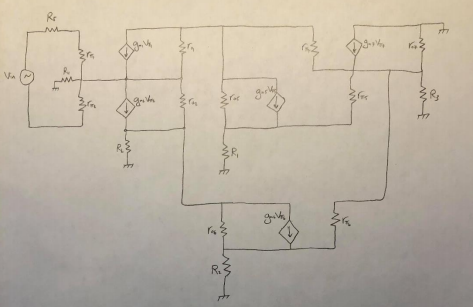
\includegraphics[width=0.7\textheight]{ssm_gain1.png}
		\captionof{figure}{Small Signal Model of The First Stage of The Gain}
		\label{f:2}
	\end{figure}
	
	\noindent\textbf{Note} that $Q_7$ is treated as a short due to the fact that there is no degeneration resistors and a single-ended load
	
	\begin{align*}
		I_5 &= \frac{v_{\pi_{5}}}{r_{o_5}} + \frac{v_{\pi_{5}}}{r_{\pi_5}} + g_{m_5} v_{\pi_{5}}\\
		&= \frac{v_{\pi_5}}{r_{o_5} // r_{\pi_{5}} // \frac{1}{g_{m_5}}} \rightarrow parallel \hspace{1mm} with \hspace{1mm} r_{\pi_{6}}
	\end{align*}
	
	\pagebreak
	A simplified small signal model of the first stage of the gain is shown below in Figure \ref{f:3}.
	\begin{figure}[!ht]
		\centering
		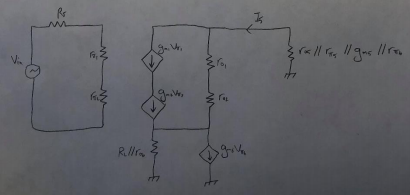
\includegraphics[width=0.7\textheight]{ssm_gain1_simplified.png}
		\captionof{figure}{Simplified Small Signal Model of The First Stage of The Gain}
		\label{f:3}
	\end{figure}
	
	\noindent In order to analyze the circuit easily, assumptions have been made:
	\begin{itemize}
		\item $r_{o_1}$ + $r_{o_2}$ is a very large so they act as an open circuit
		\item $g_{m_1} v_{\pi_1}$ and $g_{m_2} v_{\pi_2}$ can be combined since they are biased the same
		\item $g_{m_5} = g_{m_6}$ since both transistors are biased the same
		\item $R_S$ is negligible when compared to $r_{\pi_1}$ and $r_{\pi_2}$
		\item High input impedance for Stage 1
	\end{itemize}
	\begin{align*}
		V_L &= 2 g_{m_2} v_{\pi_2} (R_{L_1} // r_{o_6} // r_{o_2})\\
		A_{v_1} &= \frac{V_L}{V_{in}}\\
		&= g_{m_2} (R_{L_1} // r_{o_6} // r_{o_2})
	\end{align*}
	To determine the output resistance, a resistor equivalent is added to $R_2$:
	\begin{align*}
		R_{out_1} &= r_{o_6} [1 + g_{m_6} (R_2 // r_{\pi_6})] + (R_2 // r_{\pi_6})\\
		&= (7.90 \hspace{1mm} M\Omega) [1 + 406 \hspace{1mm}\mu A/V (1 \hspace{1mm} k\Omega // 249 \hspace{1mm} k\Omega)] + (1 \hspace{1mm} k\Omega // 249 \hspace{1mm} k\Omega)\\
		&= 11.095 M\Omega 
	\end{align*}
	Determining $R_{in}$ for the second stage of the gian:
	\begin{align*}
		R_{in_2} &= (\beta_{16} + 1) [r_{e_{16}} + r_{o_{16}} // R_9 // (r_{\pi_{17}} + R_8 + (r_{\pi_{17}}) (R_8) (g_{m_{17}}))]\\
		&= (100 + 1)[1253.13 \hspace{1mm} \Omega + 4 \hspace{1mm} M\Omega // 50 \hspace{1mm} k\Omega // (3.7 \hspace{1mm} k\Omega + 100 \hspace{1mm} \Omega + (3.7 \hspace{1mm} k\Omega)(100 \hspace{1mm} \Omega)(27.1 \hspace{1mm} \mu A/V) )]\\
		&= 1.218 \hspace{1mm} M\Omega
	\end{align*}
	Determining $R_{L_1}$:
	\begin{align*}
		R_{L_1} &= R_{in_2} // R_{out_1}\\
		&= 1.218 \hspace{1mm} M\Omega // 11.095 M\Omega\\
		&= 1.098 \hspace{1mm} M\Omega
	\end{align*}
	
	\pagebreak
	\noindent The first stage of the gain can be calculated as follows:
	\begin{align*}
		A_{v_1} &= g_{m_2} (R_{L_1} // r_{o_6} // r_{o_2})\\
		&= 414 \hspace{1mm} \mu A/V (1.098 \hspace{1mm} M\Omega // 7.90 \hspace{1mm} M\Omega // 1.93 \hspace{1mm} M\Omega)
	\end{align*}
	\begin{align*}
		\therefore A_{v_1} = 266.16 \hspace{1mm} v/v
	\end{align*}
	\subsubsection*{Stage 2 Gain ($A_{v_2}$):}
	The second stage of the gain is calculated, which is defined as the gain from the base of $Q_{16}$ to the base of $Q_{23}$.
	The small-signal model of stage 2 is shown in Figure \ref{f:4} below.
	\begin{figure}[!ht]
		\centering
		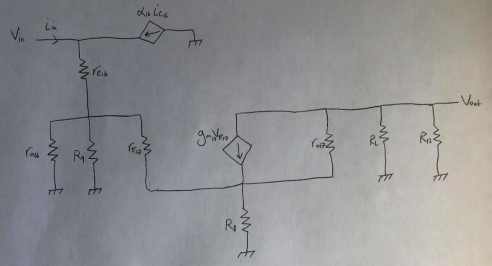
\includegraphics[width=0.8\textwidth]{ssm_gain2.png}
		\captionof{figure}{Small Signal Model of The Second Stage of The Gain}
		\label{f:4}
	\end{figure}

	\noindent The second stage of the gain can be calculated as follows:
	\begin{align*}
		A_{v_2} &= \frac{v_{out}}{v_{in}}\\
		&= \frac{v_{out}}{v_{\pi_{17}}} * \frac{v_{\pi_{17}}}{v_{b_{17}}} * \frac{v_{b_{17}}}{v_{in}}
	\end{align*}
	\begin{align*}
		\frac{v_{out}}{v_{\pi_{17}}} &= (-g_{m_{17}}) (R_{L_2} // R_{12})\\
		&= (-27.1 \hspace{1mm} mA/V)(R_{L_2} // R_{12})	
	\end{align*}
	\begin{align*}
		\frac{v_{\pi_{17}}}{v_{b_{17}}} &= \frac{r_{\pi_{17}}}{r_{\pi_{17}} + R_8(1+ \beta)}\\
		&= \frac{3.7 \hspace{1mm} k\Omega}{3.7 \hspace{1mm} k\Omega + (100 \hspace{1mm} \Omega)(1 + 100)}\\
		&= 0.2681 \hspace{1mm} v/v
	\end{align*}
	Define $r_{\pi_{17}}^{'}$ as follows:
	\begin{align*}
		r_{\pi_{17}}^{'} &= r_{\pi_{17}} + R_8(1 + \beta)\\
		&= 3.7 \hspace{1mm} k\Omega + (1 + 100) (100 \hspace{1mm} \Omega)\\
		&= 13.8 \hspace{1mm} k\Omega
	\end{align*}
	\begin{align*}
		\frac{v_{b_{17}}}{v_{in}} &= \frac{(1 + \beta)[r_{o_{16}} // R_9 // r_{\pi_{17}}^{'}]}{(1 + \beta)[r_{o_{16}} // R_9 // r_{\pi_{17}}^{'}] + r_{e_{16}} (1 + \beta)}\\
		&= \frac{(1 + 100) [4 \hspace{1mm} M\Omega // 50 \hspace{1mm} k\Omega // 13.8 \hspace{1mm} k\Omega]}{(1 + 100) [4 \hspace{1mm} M\Omega // 50 \hspace{1mm} k\Omega // 13.8 \hspace{1mm} k\Omega] + (1253.13 \hspace{1mm} \Omega)(1 + 100)}\\
		&= 0.8959 \hspace{1mm} v/v
	\end{align*}
	The input impedance of the third stage is calculated as follows:
	\begin{align*}
		R_{in_3} &= r_{e_{23}} (1 + \beta) + (1 + \beta) [(1 + \beta)[R_{10} + (r_{e_{14}} + R_6) // (r_{e_{20}} + R_7)] // R_{13}]\\
		&= (126.6 \hspace{1mm} \Omega) (1 + 100) + (1 + 100) [(1 + 100)[1 \hspace{1mm} M\Omega + (22.1 \hspace{1mm} \Omega + 30 \hspace{1mm} \Omega) // (22.1 \hspace{1mm} \Omega + 30 \hspace{1mm} \Omega)] // 90 \hspace{1mm} k\Omega]\\
		&\approx 9.095 \hspace{1mm} M\Omega
	\end{align*}
	In this stage, $R_{L_2}$ is equivalent to $R_{in_3}$
	\begin{align*}
	\therefore R_{L_2} =  9.095 \hspace{1mm} M\Omega
	\end{align*}
	Therefore, the gain for the second stage is:
	\begin{align*}
		A_{v_2}  = \left[(-27.1 \hspace{1mm} mA/V)(9.095 \hspace{1mm} M\Omega // 30 \hspace{1mm} k\Omega)\right][0.2681 * 0.8959]
	\end{align*}
	\begin{align*}
		\therefore A_{v_2} = -194.65 \hspace{1mm} v/v
	\end{align*}
	\pagebreak
	\subsubsection*{Stage 3 Gain ($A_{v_3}$):}
	The third stage of the gain is calculated.
	The small-signal model of stage 2 is shown in Figure \ref{f:5} below.
	\begin{figure}[!ht]
		\centering
		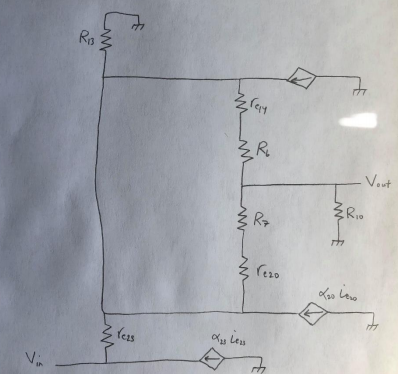
\includegraphics[width=0.7\textheight]{ssm_gain3.png}
		\captionof{figure}{Small Signal Model of The Third Stage of The Gain}
		\label{f:5}
	\end{figure}
	The third stage of the gain can be calculated as follows:
	\begin{align*}
		A_{v_3} &= \left[\frac{R_{10}}{R_{10} + (r_{e_{14}} + R_6) // (r_{e_{20}} + R_7)}\right] \left[\frac{(1 + \beta) [R_{10} + [(r_{e_{16}} + R_6) // (r_{e_{20}} + R_7) // R_{13}]]}{r_{e_{23}} + (1 + \beta) [R_{10} + [(r_{e_{16}} + R_6) // (r_{e_{20}} + R_7) // R_{13}]]} \right]\\
		&= \left[\frac{1 \hspace{1mm} M\Omega}{1 \hspace{1mm} M\Omega + (22.1 \hspace{1mm} \Omega + 30 \hspace{1mm} \Omega) // (22.1 \hspace{1mm} \Omega + 30 \hspace{1mm} \Omega)}\right] *\\
		& \hspace{4mm} \left[\frac{(1 + 100)[1 \hspace{1mm} M\Omega + [(22.1 \hspace{1mm} \Omega + 30 \hspace{1mm} \Omega) // (22.1 \hspace{1mm} \Omega + 30 \hspace{1mm} \Omega) // 30 \hspace{1mm} k\Omega]]}{126.26 \hspace{1mm} \Omega + (1 + 100)[1 \hspace{1mm} M\Omega + [(22.1 \hspace{1mm} \Omega + 30 \hspace{1mm} \Omega) // (22.1 \hspace{1mm} \Omega + 30 \hspace{1mm} \Omega) // 30 \hspace{1mm} k\Omega]]}\right]
	\end{align*}
	\begin{align*}
		\therefore A_{v_3} = 0.99 \approx 1 \hspace{1mm} v/v
	\end{align*}
	\subsubsection*{Total Gain ($G_v$):}
	Therefore, the total gain of the 741 operational amplifier can be calculated as follows:
	\begin{align*}
		G_v &= A_{v_1} * A_{v_2} * A_{v_3}\\
		&= (266.16)(-1944.65)(0.9999)\\
		&= -51.8 k \hspace{1mm} v/v
	\end{align*}
	\subsubsection*{Input Common Mode Range:}
	The maximum value of the common mode range is 4.4 V because we want to keep $Q_1$ and $Q_2$ operating in the active region.
	\begin{align*}
		V_{max} = 4.4 V
	\end{align*}
	\begin{align*}
		V_{min} &= V_{BE_1} + V_{BE_2}\\
		&= 0.6 \hspace{1mm} V + 0.6 \hspace{1mm} V\\
		&= 1.2 \hspace{1mm} V
	\end{align*}
	\subsubsection*{Output Voltage Swing:}
	\begin{align*}
		V_{max} - V_{min} &= 4.4 \hspace{1mm} V - 1.2 \hspace{1mm} V\\
		&= 3.2 \hspace{1mm} V
	\end{align*}
	\subsubsection*{Capacitor Value:}
	In order to get the unity gain frequency $f_u$ to be 1 MHz, the value of $C_1$ is determined using the following equations:
	\begin{align*}
		C_A &= C_1 (1 + A_{v_2})\\
		W_p &= \frac{1}{C_A (R_{out} // R_{in})}\\
		W_T &= A_o W_p
	\end{align*}
	\begin{align*}
		C_1 &= \frac{A_o}{2\pi f_u (1 + A_{v_2}) (R_{out} // R_{in} // r_{o_2})}\\
		&\approx 60.23 \hspace{1mm} pf
	\end{align*}
	\subsubsection*{Slew Rate:}
	\begin{align*}
		Slew \hspace{1mm} rate &= \frac{I_{C_1}}{C_1}\\
		&= \frac{19 \hspace{1mm} \mu A}{60.23 \hspace{1mm} pf}\\
		&= 0.316 \hspace{1mm} V/\mu S
	\end{align*}
	
	\pagebreak
	\section{Additional Manual Questions}
	\begin{enumerate}
		\item $V_{10}$ is the input DC voltage to the op-amp.
		It is used to set the differential voltage mode of the circuit.
		It is also used to conduct input DC voltage sweeps and input offset voltage.
		$V_5$ is used to find the common-mode input voltage which is supplied to the two input transistors $Q_1$ and $Q_2$.
		\item The purpose of $Q_7$ and $R_3$ is to act as an active load for the input of the op-amp, as well as to keep the signal stable such that the gain doesn’t change.
		Shorting the base and collector of $Q_5$ would cause $Q_{16}$ to have a large base current and could possibly cause the circuit to be unstable.
		\item The role of $C_1$ is to provide stability in the circuit and to maintain the unity-gain frequency at 1 MHz, such that a steady consistent roll-off for the circuit can occur.
		\item An ideal current source would have infinite internal resistance so that 100\% of the current from the current source can go to the load resistance.
		In a real circuit, current sources would be replaced by current mirrors.
		Thus, $R_{in}$, $R_{out}$, and the gain would differ from when using an ideal current source.
		\item The purpose of $V_2$ is to provide a stable biasing voltage to $Q_{14}$ and $Q_{20}$.
		$V_2$ would be implemented using 2 BJTs and a resistor.
		\item The purpose of the first two stages in the circuit is to achieve a high gain.
		The purpose of the third stage is to have a small load resistance value such that the high gain value is maintained.
		Splitting the circuit into three stages makes the circuit fairly easier to analyze.
		\item Assuming no input signal, the power consumption is calculated using the following euqation:
		\begin{align*}
			P = V_{CC} * I_{CC} \approx 6 \hspace{1mm} mW
		\end{align*}
	\end{enumerate}

	\pagebreak
	\section{Simulation}
	\subsection{DC Sweep}	
	After setting $C_1$ to the value found in the prelab, 60.23 pF, a DC sweep of the input differential voltage $V_d$ between -10 mV to 10 mV was done.\\
	Figure \ref{f:6} below is the transfer curve for $V_o$ versus $V_d$.
	\begin{figure}[!ht]
		\centering
		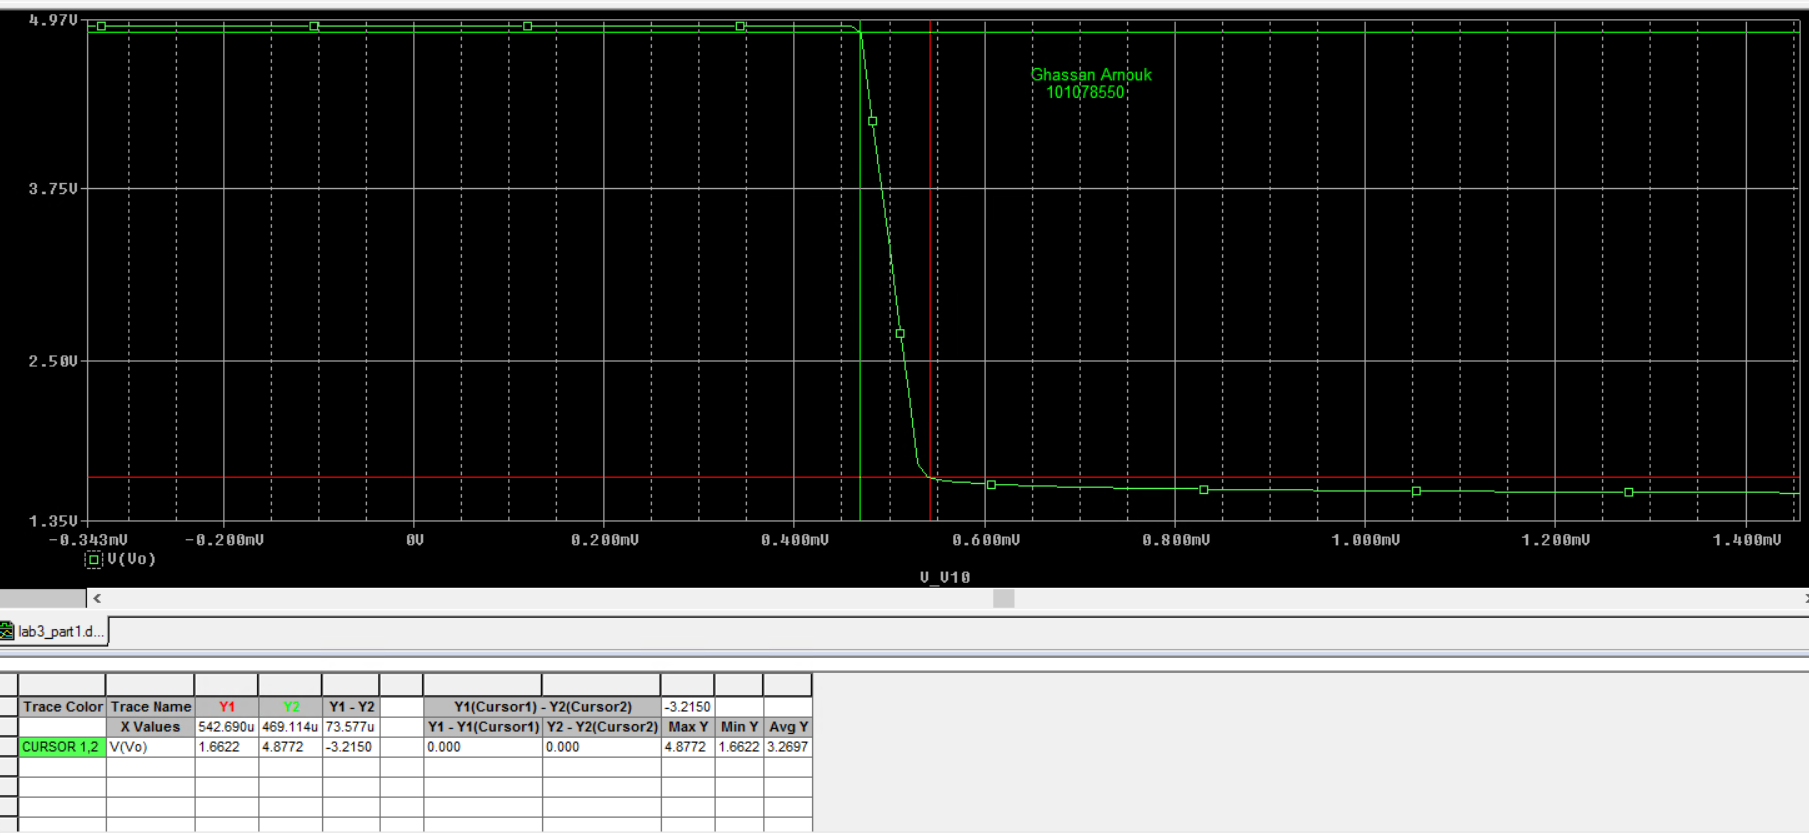
\includegraphics[width=0.7\textheight]{1.1.png}
		\captionof{figure}{Transfer Curve for $V_o$ vs. $V_D$}
		\label{f:6}
	\end{figure}

	\noindent As shown in Figure \ref{f:6}, cursors used to find the range of the linear region.
	The range of the linear region is from 1.66 V to 4.87 V.
	The output voltage swing can be calculated as follows:
	\begin{align*}
		Output \hspace{1mm} voltage \hspace{1mm} swing = 4.87 \hspace{1mm} V - 1.66 \hspace{1mm} V = 3.21 \hspace{1mm} V
	\end{align*}
	In comparison to the output voltage swing found in the prelab calculations, 3.20 V, the simulated value is very close.\\
	The differential gain is the slope of the linear region of the transfer curve. 
	Using the values at which the cursors were placed to determine the linear region range, the differential gain can be calculated as follows:
	\begin{align*}
		Differential \hspace{1mm} gain &= \frac{y_2 - y_1}{x_2 - x_1} = \frac{4.87 \hspace{1mm} V - 1.66 \hspace{1mm} V}{469 \hspace{1mm} \mu V - 543 \hspace{1mm}\mu V} = -43,378 \hspace{1mm} v/v
	\end{align*}
	The total gain calculated in the prelab was found to be -51.8 k$v/v$. 
	In comparison to the simulation value, the prelab value seems close to the simulated value.
	The difference can be attributed to the assumptions made during the calculations, such as the beta value.
	The difference can also be attributed to where the cursors on the simulation plot were place. 
	Moving the cursors wihtin the linear region would yield a different differential gain value.\\\\
	The input offset voltage, which is value of $V_d$ at which $V_o$ is 2.5 V, was found to be approximately 515 $\mu$V.
	
	\pagebreak
	\subsection{Transistor Parameters}
	For this part of the experiment, the transistor parameters for each transistor in the op-amp circuit were found.
	The simulation diagram of these parameter values are shown in Figure \ref{f:7} and can be found in the Appendix.\\\\
	Table \ref{t:3} below illustrates a comparison between the calculated and simulated transistor parameters.
	\begin{table}[!ht]
		\centering
		\captionof{table}{Calculated vs. Simulated Transistor Parameters}
		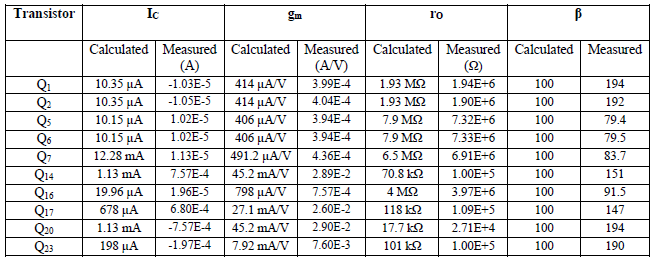
\includegraphics[width=0.7\textheight]{c_vs_s.png}
		\label{t:3}
	\end{table}
	As shown in Table \ref{t:3} above, the majority of the calculated values are very close to the simulated values.
	Any discrepancies or differences in values, such as in $I_C$ for $Q_{20}$ can be attributed to the beta value assumed for each transistor.
	Each transistor’s beta value is not a constant, and instead relies on the current.\\\\
	The gain calculations using the measured parameter values can be shown below.
	\subsubsection*{Stage 1 Gain ($A_{v_1}$):}
	\begin{align*}
		R_{in_2} &= (\beta_{16} + 1) [r_{e_{16}} + r_{o_{16}} // R_9 // (r_{\pi_{17}} + R_8 + (r_{\pi_{17}}) (R_8) (g_{m_{17}}))]\\
		&= (91.5 + 1)[1321 \hspace{1mm} \Omega + 3.97 \hspace{1mm} M\Omega // 50 \hspace{1mm} k\Omega // (5.65 \hspace{1mm} k\Omega + 100 \hspace{1mm} \Omega + (5.65 \hspace{1mm} k\Omega)(100 \hspace{1mm} \Omega)(0.26 \hspace{1mm} mA/V))]\\
		&= 1.459 \hspace{1mm} M\Omega
	\end{align*}	
	\begin{align*}
		R_{out_1} &= r_{o_6} [1 + g_{m_6} (R_2 // r_{\pi_6})] + (R_2 // r_{\pi_6})\\
		&= (7.33 \hspace{1mm} M\Omega) [1 + 394 \hspace{1mm}\mu A/V (1 \hspace{1mm} k\Omega // 202 \hspace{1mm} k\Omega)] + (1 \hspace{1mm} k\Omega // 202 \hspace{1mm} k\Omega)\\
		&= 10.071 \hspace{1mm} M\Omega 
	\end{align*}	
	\begin{align*}
		R_{L_1} &= R_{in_2} // R_{out_1}\\
		&= 1.459 \hspace{1mm} M\Omega // 10.071 \hspace{1mm} M\Omega\\
		&\approx 1.247 \hspace{1mm} M\Omega
	\end{align*}
	\begin{align*}
		A_{v_1} &= \frac{v_L}{v_{in}}\\
		&= g_{m_2} (R_{L_1} // r_{o_6} // r_{o_2})\\
		&= 404 \hspace{1mm} \mu A/V (1.247 \hspace{1mm} M\Omega // 7.33 \hspace{1mm} M\Omega // 1.90 \hspace{1mm} M\Omega)
	\end{align*}
	\begin{align*}
		\therefore A_{v_1} = 279.07 \hspace{1mm} v/v
	\end{align*}
	
	\pagebreak
	\subsubsection*{Stage 2 Gain ($A_{v_2}$):}
	\begin{align*}
		A_{v_2} &= \frac{v_{out}}{v_{in}}\\
		&= \frac{v_{out}}{v_{\pi_{17}}} * \frac{v_{\pi_{17}}}{v_{b_{17}}} * \frac{v_{b_{17}}}{v_{in}}
	\end{align*}
	\begin{align*}
		\frac{v_{out}}{v_{\pi_{17}}} &= (-g_{m_{17}}) (R_{L_2} // R_{12})\\
		&= (-26 \hspace{1mm} mA/V)(R_{L_2} // 30 \hspace{1mm} k\Omega)	
	\end{align*}
	\begin{align*}
		\frac{v_{\pi_{17}}}{v_{b_{17}}} &= \frac{r_{\pi_{17}}}{r_{\pi_{17}} + R_8(1+ \beta)}\\
		&= \frac{5.63 \hspace{1mm} k\Omega}{5.63 \hspace{1mm} k\Omega + (100 \hspace{1mm} \Omega)(1 + 147)}\\
		&= 0.2756 \hspace{1mm} v/v
	\end{align*}
		Define $r_{\pi_{17}}^{'}$ as follows:
	\begin{align*}
		r_{\pi_{17}}^{'} &= r_{\pi_{17}} + R_8(1 + \beta)\\
		&= 5.63 \hspace{1mm} k\Omega + (1 + 147) (100 \hspace{1mm} \Omega)\\
		&= 20.43 \hspace{1mm} k\Omega
	\end{align*}
	\begin{align*}
		\frac{v_{b_{17}}}{v_{in}} &= \frac{(1 + \beta)[r_{o_{16}} // R_9 // r_{\pi_{17}}^{'}]}{(1 + \beta)[r_{o_{16}} // R_9 // r_{\pi_{17}}^{'}] + r_{e_{16}} (1 + \beta)}\\
		&= \frac{(1 + 91.5) [3.97 \hspace{1mm} M\Omega // 50 \hspace{1mm} k\Omega // 20.43 \hspace{1mm} k\Omega]}{(1 + 91.5) [3.97 \hspace{1mm} M\Omega // 50 \hspace{1mm} k\Omega // 20.43 \hspace{1mm} k\Omega] + (1321 \hspace{1mm} \Omega)(1 + 91.5)}\\
		&= 0.9162 \hspace{1mm} v/v
	\end{align*}
	The input impedance of the third stage is calculated as follows:
	\begin{align*}
		R_{in_3} &= r_{e_{23}} (1 + \beta_{23}) + (1 + \beta_{23}) [(1 + \beta_{14})[R_{10} + (r_{e_{14}} + R_6) // (r_{e_{20}} + R_7)] // R_{13}]\\
		&= (131.58 \hspace{1mm} \Omega) (1 + 190) + (1 + 190) [(1 + 151)[1 \hspace{1mm} M\Omega + (60.6 \hspace{1mm} \Omega // 64.48 \hspace{1mm} \Omega)] // 90 \hspace{1mm} k\Omega]\\
		&\approx 17.205 \hspace{1mm} M\Omega
	\end{align*}
		In this stage, $R_{L_2}$ is equivalent to $R_{in_3}$
	\begin{align*}
		\therefore R_{L_2} =  17.205 \hspace{1mm} M\Omega
	\end{align*}
	\begin{align*}
		\frac{v_{out}}{v_{\pi_{17}}} &= (-g_{m_{17}}) (R_{L_2} // R_{12})\\
		&= (-26 \hspace{1mm} mA/V)(17.205 \hspace{1mm} M\Omega // 30 \hspace{1mm} k\Omega)\\
		&= -778.64 \hspace{1mm} v/v
	\end{align*}	
	Therefore, the gain for the second stage is:
	\begin{align*}
		A_{v_2} = (-778.64)(0.2756)(0.9162)
	\end{align*}
	\begin{align*}
		\therefore A_{v_2} = -196.60 \hspace{1mm} v/v
	\end{align*}
	
	\pagebreak
	\subsubsection*{Stage 3 Gain ($A_{v_3}$)}
	\begin{align*}
		A_{v_3} &= \left[\frac{R_{10}}{R_{10} + (r_{e_{14}} + R_6) // (r_{e_{20}} + R_7)}\right] \left[\frac{(1 + \beta_{14}) [R_{10} + [(r_{e_{16}} + R_6) // (r_{e_{20}} + R_7) // R_{13}]]}{r_{e_{23}} + (1 + \beta_{14}) [R_{10} + [(r_{e_{16}} + R_6) // (r_{e_{20}} + R_7) // R_{13}]]} \right]\\
		&= \left[\frac{1 \hspace{1mm} M\Omega}{1 \hspace{1mm} M\Omega + (64.6 \hspace{1mm} \Omega) // (64.48 \hspace{1mm} \Omega)}\right] *\\
		& \hspace{4mm} \left[\frac{(1 + 151)[1 \hspace{1mm} M\Omega + [(64.6 \hspace{1mm} \Omega) // (64.48 \hspace{1mm} \Omega) // 90 \hspace{1mm} k\Omega]]}{131.58 \hspace{1mm} \Omega + (1 + 151)[1 \hspace{1mm} M\Omega + [(64.6 \hspace{1mm} \Omega) // (64.48 \hspace{1mm} \Omega) // 90 \hspace{1mm} k\Omega]]}\right]
	\end{align*}
	\begin{align*}
		\therefore A_{v_3} = 0.9999 \approx 1 \hspace{1mm} v/v
	\end{align*}
	\subsubsection*{Total Gain ($G_v$):}
	Therefore, the total gain of the 741 operational amplifier can be calculated as follows:
	\begin{align*}
		G_v &= A_{v_1} * A_{v_2} * A_{v_3}\\
		&= (279.07)(-196.60)(0.9999)\\
		&= -54,864 \hspace{1mm} v/v
	\end{align*}
	\begin{table}[!ht]
		\centering
		\captionof{table}{Prelab vs. Simulated Voltage Gains}
		\begin{tabular}{|c|c|c|}
			\hline
			Stage Gain & Prelab Gain & Simulated Gain\\
			\hline\hline
			$A_{v_1}$ & 266.16 $v/v$ & 279.07 $v/v$\\
			\hline
			$A_{v_2}$ & -194.65 $v/v$ & -196.60 $v/v$\\
			\hline
			$A_{v_3}$ & 0.9999 $v/v$ & 0.99997 $v/v$\\
			\hline
			$G_v$ & -51,800 $v/v$ & -54,863 $v/v$\\
			\hline
		\end{tabular}
		\label{t:4}
	\end{table}
	As shown in Table \ref{t:4}, the gain values from the prelab come very close to the gain values using the simulation determined parameters.
	The difference between the gains can again be attributed mainly to the different beta values determined by the simulation.
	They make significant differences when used in the calculations. 
	Also, in the simulation, $I_B$ is not assumed to be zero.
	In the prelab, $I_B$ was assumed to be zero in order to ease the calculations. 
	The accuracy of the calculations in the prelab are less when compared to the simulated results.
	This is due to the fact that assumptions were made when doing the prelab calculations, whereas the simulation is very accurate in its data.
	
	\pagebreak
	\subsection{DC Sweep from 0V to 5V}
	Another DC sweep was done, set from 0 V to 5 V, and the differential voltage $V_d$ was set to the input offset voltage, which in this case was approximately 515 $\mu$V.\\
	The transfer curve of $V_o$ vs. $V_{cm}$ is shown in Figure \ref{f:8} below.
	\begin{figure}[!ht]
		\centering
		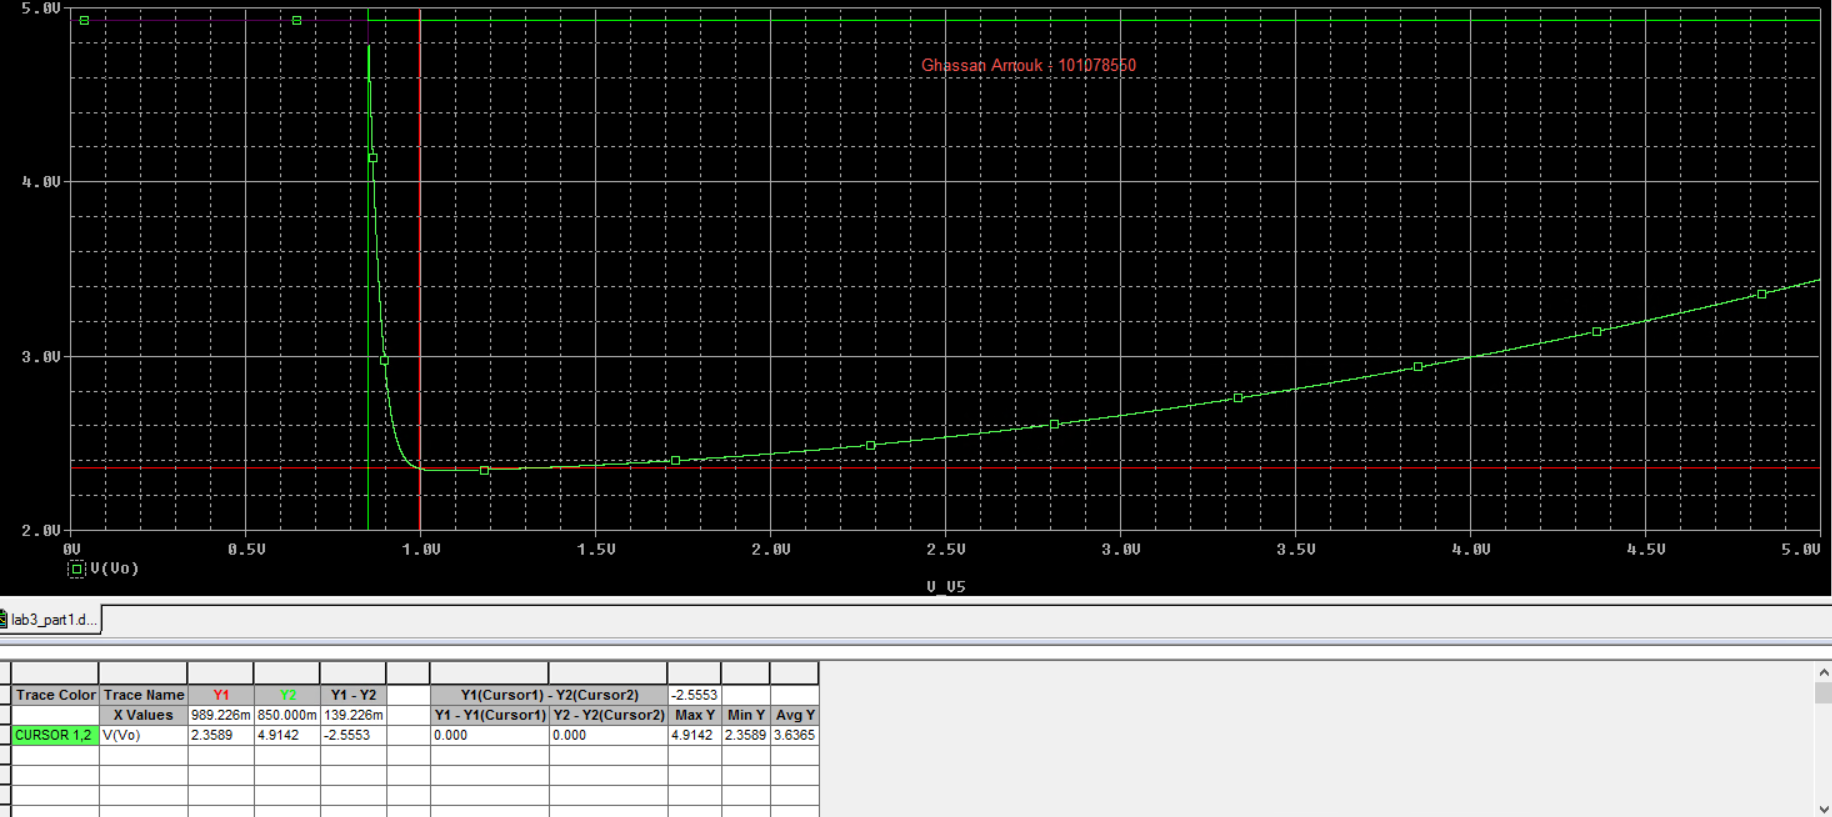
\includegraphics[width=\textwidth]{1.3.png}
		\captionof{figure}{Transfer Curve of $V_o$ vs. $V_{cm}$}
		\label{f:8}
	\end{figure}

	\noindent As shown in Figure \ref{f:8}, the common-mode range starts from 1 V and progresses onwards to 5 V. 
	Due to the fact that 5 V is the maximum value for the sweep, the plot cannot go any further. 
	This range is expected and is very close to the common-mode range determined in the prelab.
	
	\pagebreak
	\subsection{Slew Rate}
	The maximum rate-of-change of the output voltage is known as the slew rate. 
	In order to measure it, the op-amp is set to the unity-gain voltage-follower configuration.
	The positive and negative slew rates are shown in the input and output transient voltage waveforms in Figure \ref{f:9} and Figure \ref{f:10} below.\\
	Figure \ref{f:9} illustrates the use of cursors to measure the positive slew rate while Figure \ref{f:10} illustrates the use of cursors to measure the negative slew rate.
	\begin{figure}[!ht]
		\centering
		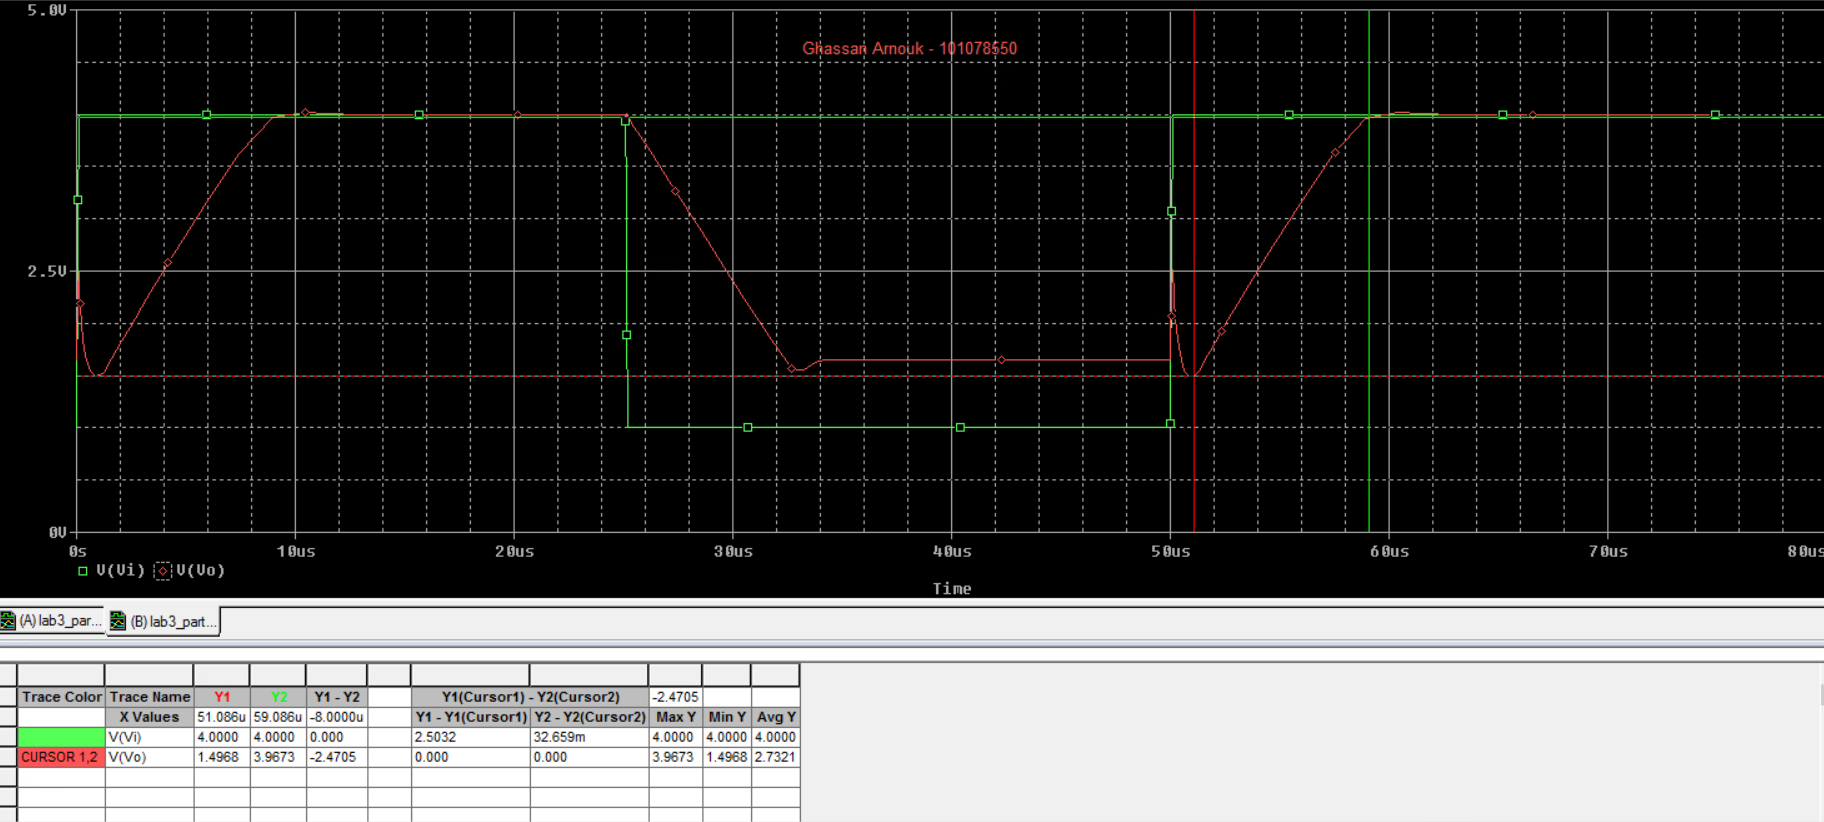
\includegraphics[width=0.7\textheight]{2.2.png}
		\captionof{figure}{Positive Slew Rate Transient Waveform}
		\label{f:9}
	\end{figure}
	\begin{figure}[!ht]
		\centering
		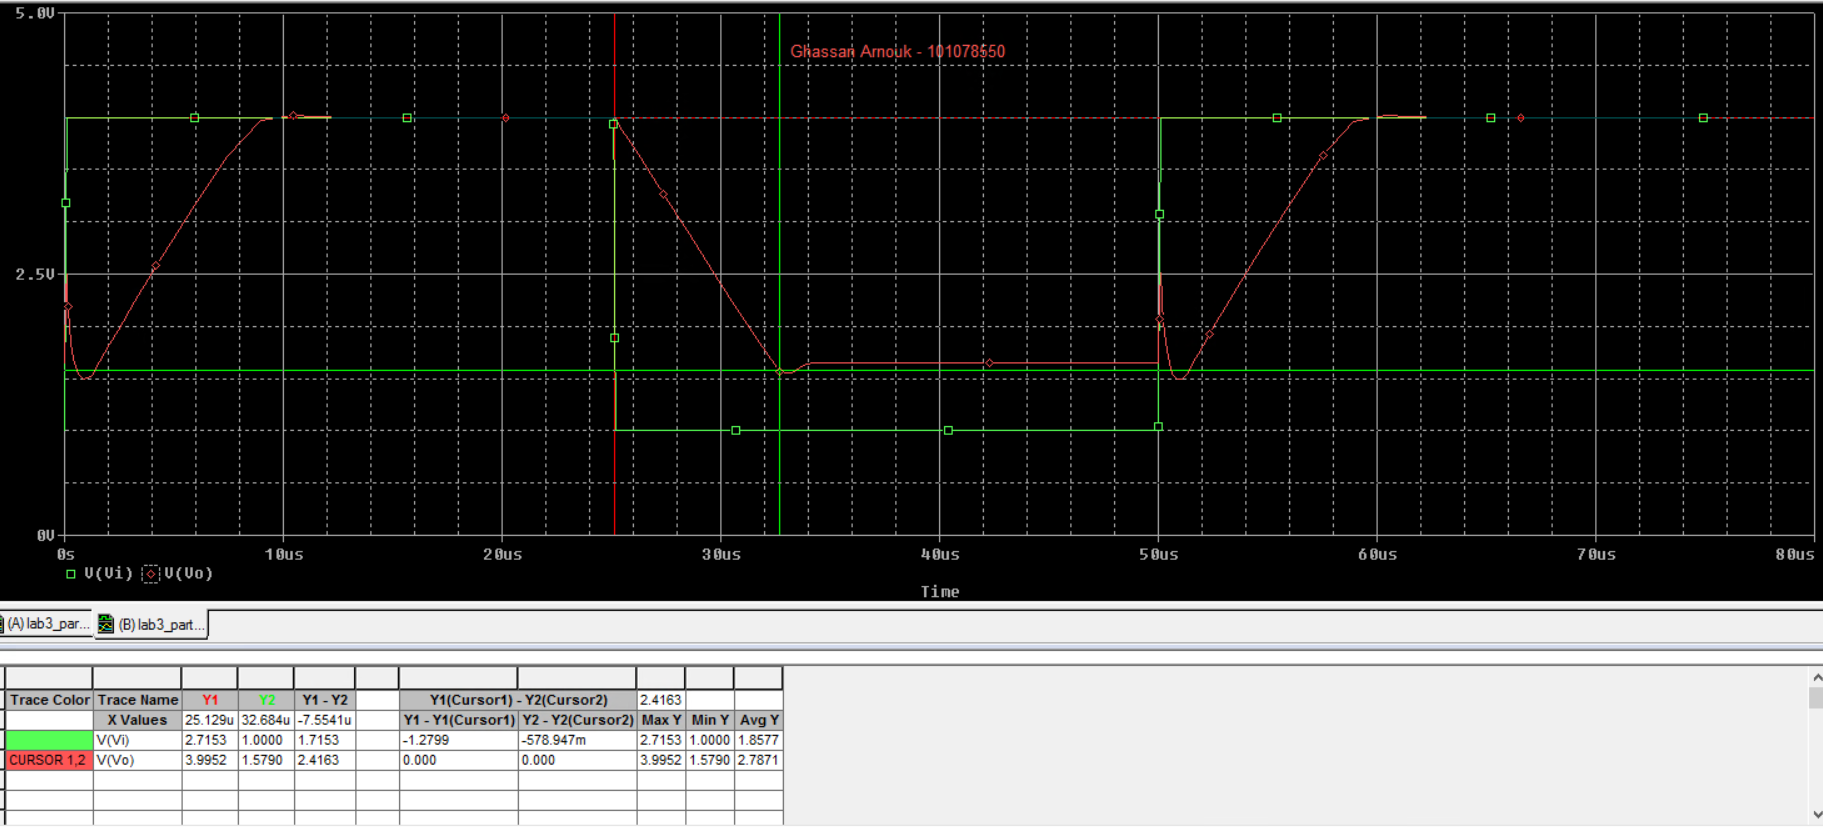
\includegraphics[width=0.7\textheight]{2.1.png}
		\captionof{figure}{Negative Slew Rate Transient Waveform}
		\label{f:10}
	\end{figure}

	\pagebreak
	\noindent As shown in Figure \ref{f:9} and Figure \ref{f:10}, the cursors are used to determine the range over which the positive and negative slew rates can be found respectively.\\
	The positive and negative slew rate calculations can be done as follows:
	\begin{align*}
		Positive \hspace{1mm} slew \hspace{1mm} rate &= \frac{\Delta y}{\Delta x}\\
		&= \frac{-2.4705 \hspace{1mm} V}{-8.0 \hspace{1mm} \mu\sec}\\
		&\approx 0.309 \hspace{1mm} V/\mu\sec
	\end{align*}
	\begin{align*}
		Negative \hspace{1mm} slew \hspace{1mm} rate &= \frac{\Delta y}{\Delta x}\\
		&= \frac{2.4163 \hspace{1mm} V}{-7.5541 \hspace{1mm} \mu\sec}\\
		&\approx -0.319 \hspace{1mm} V/\mu\sec
	\end{align*}	
	In comparison between the value of the slew rate determined in the prelab, 0.316 $V/\mu\sec$, and calculated one, it is shown that the values are very close. 
	Thus, the prelab calculations were done correctly and the correct capacitor value was chosen.
	\subsection{Frequency Response}
	In this part of the experiment, an AC sweep was done from 1 Hz to 10 MHz and Figure \ref{f:11} below shows the plot of the magnitude and phase, top and bottom respectively.
	\begin{figure}[!ht]
		\centering
		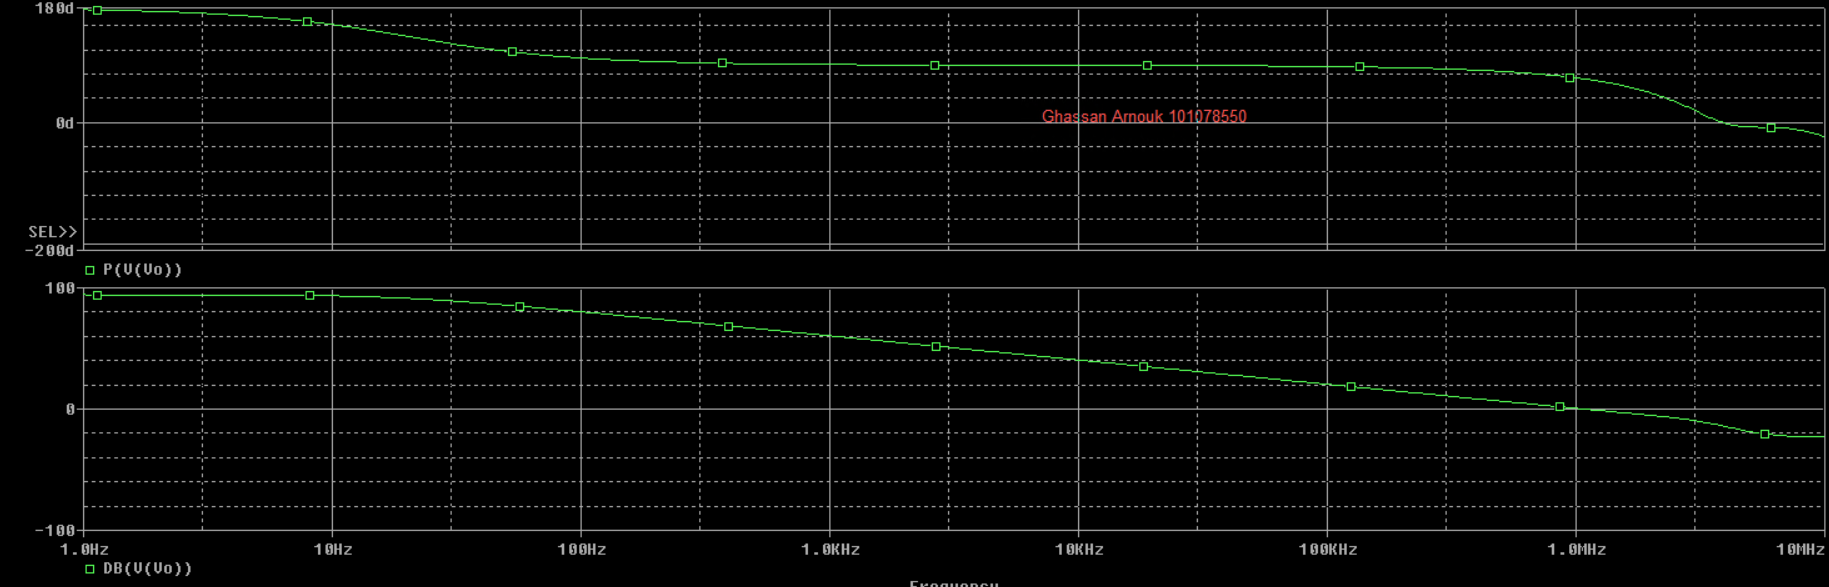
\includegraphics[width=0.7\textheight]{3.0.png}
		\captionof{figure}{Magnitude and Phase Response Plots of the 741 Op-Amp Circuit}
		\label{f:11}
	\end{figure}
	
	\noindent In order to determine the unit gain frequency $f_u$, the magnitude response was zoomed into to determine at what frequency the plot crosses zero on the y-axis as shown in Figure \ref{f:12}.
	
	\pagebreak
	\begin{figure}[!ht]
		\centering
		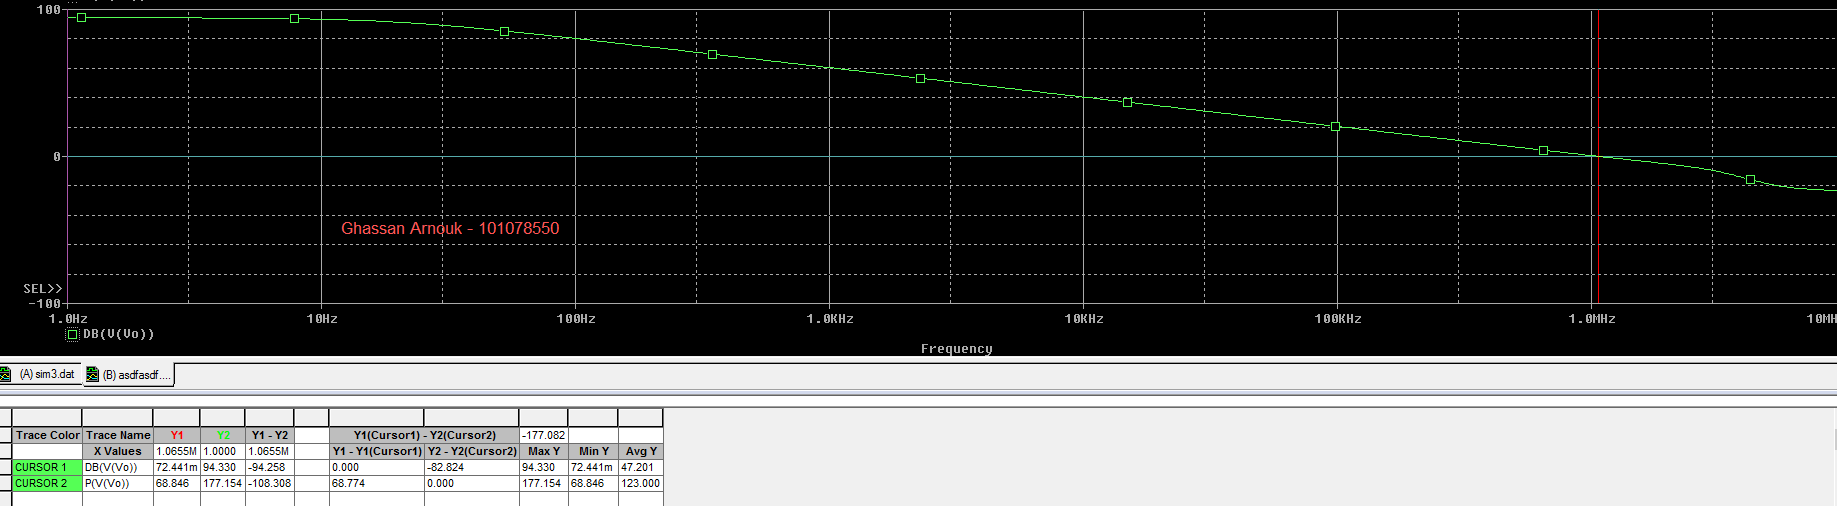
\includegraphics[width=0.7\textheight]{3.1.png}
		\captionof{figure}{Zoomed in Magnitude Response Plot}
		\label{f:12}
	\end{figure}
	\noindent Using the cursors in Figure \ref{f:12}, it is seen that the unity gain frequency is 1.0655 MHz. 
	In comparison to the 1 MHz value found in the prelab, the simulated value is very close. 
	This plot confirms that the capacitor value chosen from the prelab is correct.
	
	\pagebreak
	\section{Conclusion}
	This lab allowed us to analyze the 741 op-amp in detail. We were able to calculate and determine the calculated and simulated op-amp’s transistor parameters. As well, We were able to determine various factors of the op-amp, such as the common-mode range and the slew rate. We were also able to observe the magnitude at which this op-amp can amplify signals. Finally, this lab allowed us to get hands on experience with the simulation software, which will be very useful in further academic and professional endeavours.
	
	\pagebreak
	\section{References}
	[1] “Lab 3: 741 Op-Amp,” Carleton Univeristy, Ottawa, 2017.
	
	\pagebreak
	\section{Appendix}
	\begin{figure}[!ht]
		\centering
		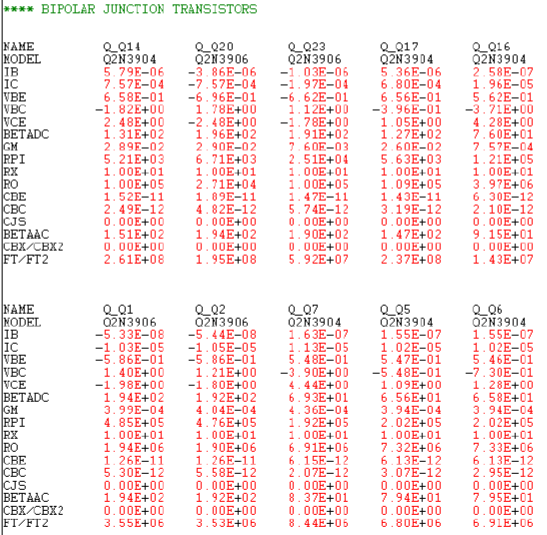
\includegraphics[width=0.6\textheight]{1.2.png}
		\captionof{figure}{Simulated Transistor Parameters}
		\label{f:7}
	\end{figure}

\end{document}